\documentclass[11pt]{article}
	\usepackage[font={small}]{caption}
	\usepackage{graphicx}
	\usepackage{xcolor}
	\usepackage{pdfpages}
	\usepackage{hyperref}
	\hypersetup{
		colorlinks,
		linkcolor={red!50!black},
		citecolor={blue!50!black},
		urlcolor={blue!80!black}
		}

%opening
\title{What a Mouse can teach Computer Science: \\
	a Computational Account of Reversal Learning.}
\author{H\'ector J. V\'azquez Mart\'inez}

\begin{document}

\maketitle

\begin{abstract}
	
I propose a computational account of the tactile discrimination reversal learning task, named the Context Grounding Hierarchy, and propose to use it to both characterize and explain the learning behavior exhibited by mice.

In order to bridge the gap between the biological learning observed in mice and reinforcement learning, it is necessary to develop a computational account of learning that observes the biological and computational constraints exhibited by the mouse brain and establishes a series of principles to design further reinforcement learning models.

I have taken steps toward this goal by identifying the computational constraints exhibited by mice and summarizing them in the Context Grounding Hierarchy.  I then affirm the effectiveness of the Context Grounding Hierarchy by using it to explain discrepancies between the performance of a state of the art reinforcement learning model trained to perform reversal learning and the performance of mice.  Finally, I propose multiple in-depth research directions necessary to confirm this principle and provide a novel approach to account for context changes in the framework of reinforcement learning.
\end{abstract}


\section{Vision}

The tactile discrimination reversal learning task performed by head-restrained mice has elucidated many key cognitive functions that seem to be in agreement with current  Reinforcement Learning techniques.  More specifically, distributed representations of sensory data, perceived reward. reward prediction and reward prediction errors have been identified in different parts of the mouse brain and observed to change as the mice subjects acquire expert-level performance in the discrimination task. 

I propose the Context Grounding Hierarchy as a set of principles for the design and implementation of Reinforcement Learning models that observe the separation of these task-specific computations.  Moreover, I partition the learning process into three major faculties: the mapping from inputs to outputs, the valuation of the input-output mapping according to reward feedback and the fulfillment of developed expectation.  The three faculties are individually represented by the levels of the Context Grounding Hierarchy: the Reaction Level, the Evaluation Level and the Expectation Level.  By the end of this paper, you will have an in depth understanding of what each of these levels is, the computational and biological constraints positing them, their interactions and how this framework can be applied to reinforcement learning.

\subsection{Mice demonstrate computational constraints.}

The tactile discrimination experiment involves stochastically presenting 2 different types of sandpaper (P100 and P1200) to head-restrained mice.  They must, in turn, use their whiskers to explore and learn to recognize each of these textures individually.  A specified time after each texture has been presented and removed, the mice must choose whether to select or reject the presented texture by either licking a water spout, or actively withholding from it.  Each combination of texture and active selection is associated with either a reward or punishment.  On the other hand, when mice withhold from licking, they reject the presented texture, but do not receive any sort of feedback from the experimental setup.  Once mice achieve expert level performance (90\%), the contingency of positively- and negatively-rewarded combinations of texture and licking are flipped, starting the reversal learning portion of the experiment.

Through the tactile discrimination experiment, intermingled representations of touching, whisking and licking have been found between the primary (S1) and secondary (S2) somatosensory areas and the vibrissae motor cortex (M1).  These representations were also observed to partially reorganize as the discrimination task was learned (F. Helmchen et. al, 2018).  It may be argued that the naive learning phase is mostly supported by these cortico-cortical interactions, allowing the mice to map a sensory input to the desired output.

Once the mice have reached expert level performance, the reversal of the texture to output contingency must then be managed by a higher order cognitive structure that will not simply forget the initially learned rule.  Mice who have been afflicted with lesions to the orbitorfrontal cortex (OFC) exhibit very similar performance to healthy mice in the initial learning phase of the experiment, but then are much slower to reacquire expert level performance after the contingency has been flipped.  For this reason, it is hypothesized that this higher level task is managed by the OFC, which encodes the task state space via many aspects of task information, including reward value, probability, risk, information value, abstract rules, and strategies (Zhang, et. al, 2018).  However, even thought the OFC has been made one of the direct drivers of learning by computing reward prediction errors directly, it has been demonstrated that neurons in the OFC signal reward prediction, not reward prediction errors (Stalnaker, et. al, 2018).

Experimental observations hint at a distributed computation of positive and negative reward values for each input-output pair, as well as their stabilization in memory as attractors.  Projections from the OFC to the Nucleus Accumbens evaluate negative outcomes of actions, while the Amygdala's projections to the OFC evaluate positively rewarded actions.  Finally, the circuit from the OFC to the Amygdala stabilizes the learned action values from the other two circuits (SM Groman, et. at, 2019).

\section{The Context Grounding Hierarchy provides steps towards the computation of Context.}
The Context Grounding Hierarchy derives its name by connecting (grounding) the computation of context directly to the information received from the external environment.  It is a pipeline of information that starts in the external environment through both stimuli and rewards, and flows up to higher level functions, such as the detection in changes of context (\autoref{fig:1}).

I will now explicitly define the Context Grounding Hierarchy as illustrated by currently known biological constraints and address its overlap with current Actor-Critic methods in Reinforcement Learning.  

\begin{figure}
	\centering
	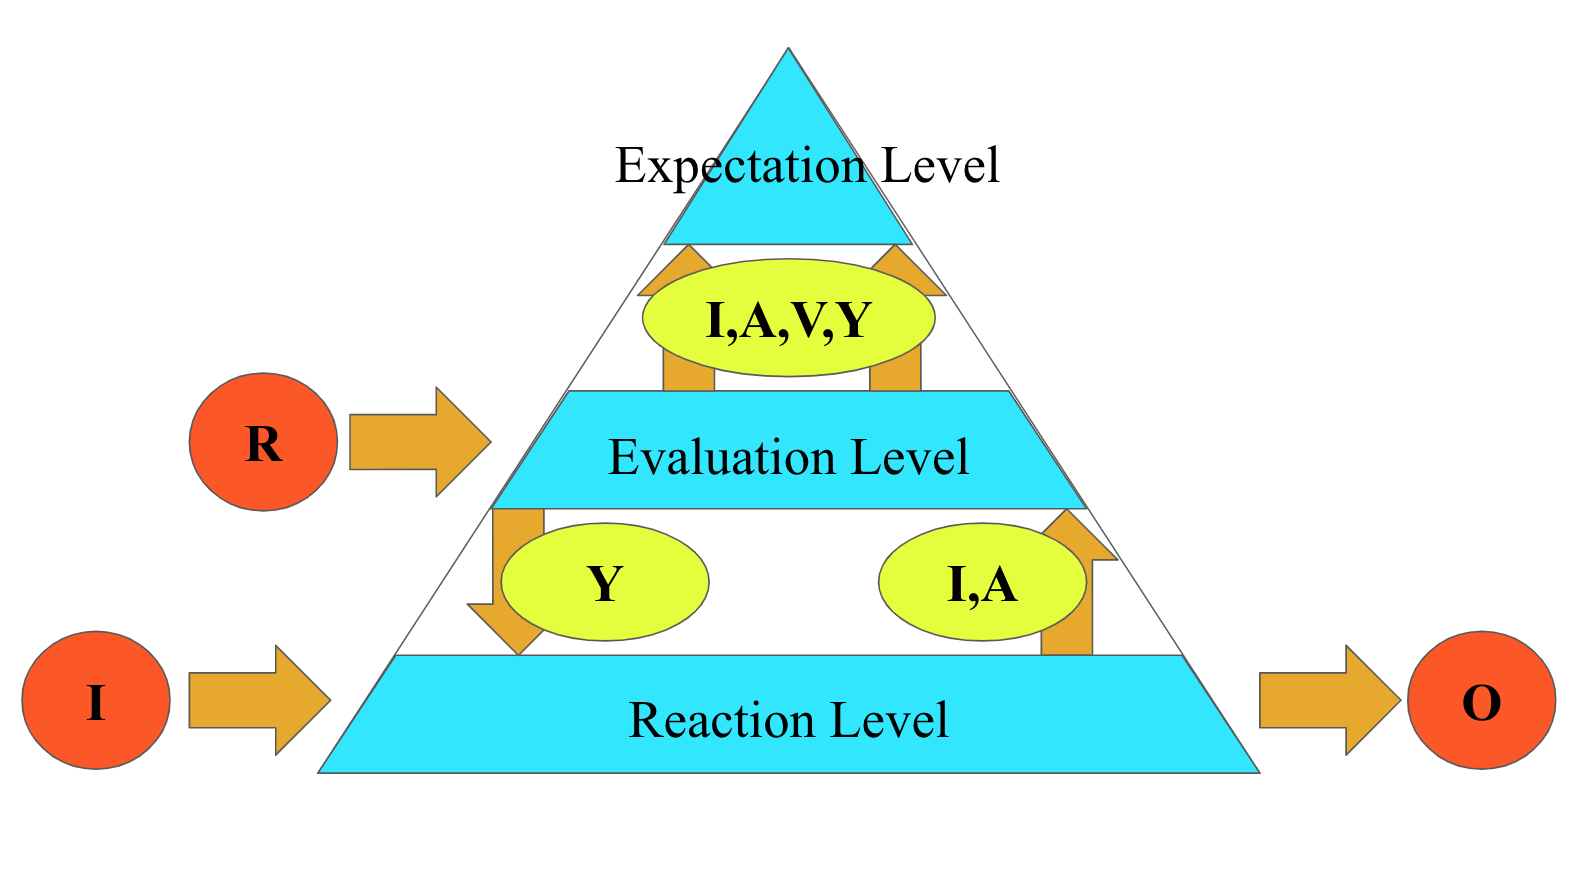
\includegraphics[scale=0.4]{./context_grounding_hierarchy.png}
	\caption{A simplified diagram of the Context Grounding Hierarchy.  Elements coming from or going to the model's environment are represented in red: Input (I), Output (O), Reward (R).  The Input comes directly into the Reaction Level, which outputs a response Action and feeds the Input-Action pair (I, A) up to the Evaluation Layer.  The Reaction Layer then updates its weights using the teaching signal (Y) coming from the Evaluation Layer.  The Evaluation Layer updates the value of the Input-Action pair according to the received Reward and feeds the updated value (V), the Input-Action pair and the teaching signal forward (I, A, V, Y) to the Expectation Layer.  The Expectation Layer then uses discrepancies between high or low values and the teaching signal to shift the axes of the Input-Action-Value function. }
	\label{fig:1}
\end{figure}


\subsection{The Reaction Level maps sensory input to an output action.}
The Reaction Level describes a naive input to output mapping.  Its simplest description is a rudimentary set of weights that map a given input to a specific output, such as in a shallow neural network.  When no learning has occurred, this mapping is entirely random. When the Reaction Level receives an external, environmental input, it produces an output action and provides the chosen input-output pair to the Evaluation Layer.  Upon receiving a learning signal ($Y$ or $Y_{true}$) as feedback from the Evaluation Level, the weights connecting the input directly to the produced output will either be strengthened or weakened according to the value of the outcome.

\subsection{The Evaluation Level attributes value to each input-output response.}
The Evaluation Level is responsible for handling the administered rewards and punishments.  In this layer, the reward or punishment signal is received, as well as the input and chosen action pair $(I, A)$ from the Reaction Level.  According to a certain learning rate, the input-output pairs provided by the Reaction Level will slowly build either a positive or negative value according to the reward received at each iteration.

A common issue is that such feedback signals are typically not a binary 1 or -1, but instead span a continuous spectrum which varies by how much reward or punishment was administered, how strong it was and how much it was needed or desired.  For example, a dehydrated mouse in the tactile discrimination experiment will highly value any water droplets administered as reward through the water spout when it chooses the right texture.  Typically, such a reward is modeled as $r = 1$.  In contrast, an unpleasant sound played when the mouse chooses the incorrect texture will commonly equate either $r = 0$ or $r = -1$ in a weight update equation.  It is incorrect to equate the magnitude of both when updating weights, even when the learning rates for positive and negative updates are different, because much needed water and an unpleasant sound are fundamentally perceived very differently.

The Evaluation Level allows the abstraction of this entire spectrum away from the hierarchy by only providing a binary learning signal $Y_{true}$ to the other levels.  This means the Reaction Level is not concerned with reward, and only concerned with the correct input to output mapping.  The Evaluation level provides, in addition to the input-action pair $(I, A)$, the value $V$ (or predicted reward $R_{pred}$) associated with it to the Expectation Level, along with the learning signal.

\subsection{The Expectation Level uses surprises to remap the input-output-value function.}
The Expectation Level then receives a function mapping input-output pairs to a predicted reward value $f(I, A) = R_{pred}$, as well as the feedback signal $Y_{true}$ which would indicate whether the predicted value is correct or not.  The function $f(-)$ received by the Expectation Layer creates a multi-dimensional surface plot by using the input, action and reward as the axes.  The learning signal indicates whether the current value function agrees with the current state of the task.  When the predicted reward $R_{pred}$ of an input-action pair $(I, A)$ is sufficiently high (or low), but the learning signal $Y_{true}$ indicates otherwise, this is taken to be surprising to the model.  The difference between the learning signal and the predicted reward may then be used as parameters to calculate a change of coordinate space of the value function in order to once again accurately describe the context.  

One such example of this operation would be to rotate the Input-Action axes by a factor of $\frac{\pi}{2}$ when the texture-action contingency is reversed with the model already at expert level performance (90\%).  This would cause the model to flip the positive and negative values attributed to each texture in the Evaluation Layer, which would then cascade to the Reaction Level through the learning signal.

\subsection{The three levels are more specific than Actor-Critic architectures.}

The typical Actor-Critic architecture in Reinforcement Learning is composed of an Actor which is mainly defined as the Reaction Level, and a Critic which encompasses the functions of the Evaluation and Expectation Level.  In traditional Actor-Critic architectures that rely on a probability distribution, usually as a softmax, as an intentioned choice model, the probability for each potential output is taken as the expectation $E[r]$ of the model.  The Critic then performs some variation of Temporal Displacement (TD) learning in the weight update rule with an $(r - E[r]])$ term.  

The Context Grounding Hierarchy separates the computation of expectation from that of the final output action.  Instead, the expectation is handled in the Evaluation Layer as a progressive accumulation of the full reward information according to a certain discount factor, while the probabilistic precursor to action selection in the Reaction Level is considered the confidence behind the action.  Having a weight plasticity rule that takes into account this confidence $c$ such as $(Y_{true} - c)$ would allow the learning to saturate and control the magnitude of the input-output weights without the need to normalize them.

\section{News}
I will now discuss my progress to date with the current state of the art model of the Orbitofrontal Cortex (OFC) (Zhang, et. al, 2018).  I will compare my own findings and discuss limitations in light of the Context Grounding Hierarchy.

\subsection{A reservoir neural network may model the OFC.}
At the time of writing, a recent publication attempting to model the mice tactile discrimination reversal learning task was by Zhang, et. al, who presented a reservoir neural network model of the OFC (\autoref{fig:2}).  In their paper, they described a reservoir which received as input a texture represented by a 2-dimensional binary vector, and a binary reward variable which represented the reward earned in the previous trial.  The network output consisted of two nodes, representing two possible actions.  In each trial, one of the two nodes would be selected and set to 1, while the other was set to 0.  This represented the choice between licking and not licking, or go vs. no-go.  The only plastic weights in the entire network were the output weights, which constitute a linear readout of the output of the reservoir.  These were updated through a Hebbian Learning rule.

\begin{figure}
	\centering
	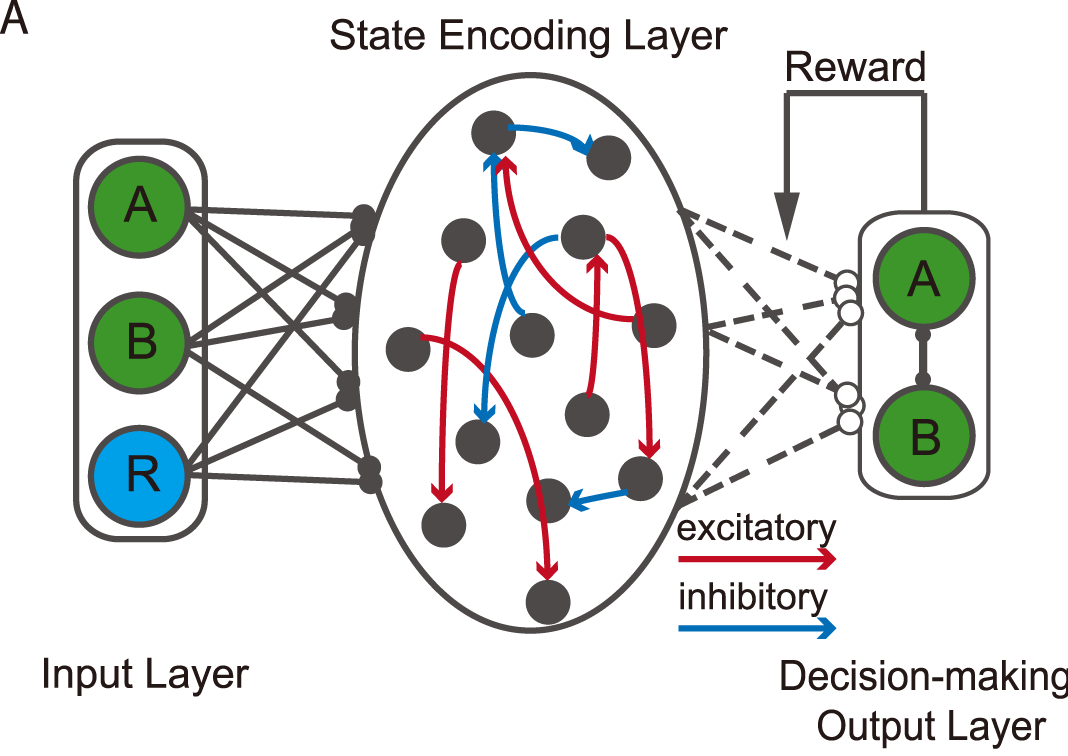
\includegraphics[scale=0.25]{./zhang_reservoir_architecture.PNG}
	\caption{A diagram of Zhang et. al's reservoir neural network model of the orbitofrontal cortext (OFC).}
	\label{fig:2}
\end{figure}

According to their findings, the reservoir network was able to learn the initial contingency, but upon reversal would first need time to forget the first learned set of weights in the output layer, making the reversal learning phase slower.  It was not until they included the reward from the previous trial into the input of the reservoir that they were able to achieve a faster reversal learning phase.  Moreover, each subsequent reversal of the texture-reward contingency was learned even faster than the previous one.  Much like the mice, they argued, the reservoir network model learned an initial task structure and later became adept at simply switching the contingency without forgetting the previously learned rewarded rule.

\subsection{The Context Grounding Hierarchy explains limitations.}
According to the paper published by Zhang et. al, the output of the model is calculated by taking a softmax of both output nodes connected to the reservoir.  The probabilities obtained from this function are then considered the expected rewards $E[r_k]$ of each function.  The plasticity equation  then uses this term in a TD-style term: $(r - E[r_k]))$.  It is not mentioned how the reservoir is able to reverse the learned contingency, aside from it being computed abstractly in the temporal dynamics of the pooled neurons.

I have implemented the network as described in their paper in iPython notebooks (see Supplementary Materials 1:1.3) using all the provided hyperparameters and an identical trial structure.  I have not yet been able to replicate the results presented in the paper.  Instead, I have discovered the following behaviors:
- Inclusion of the reward from the previous trial hinders learning.  Without knowing the action associated to a previous reward, including it as an input does not offer any further information regarding the task structure, and only serves to make the input noisier.
- Reversals are slower than the initial learning, both with and without the old reward input.  Because the weights are normalized upon initialization and with every update, the initial weights do not cause the initial learning to be any slower than later reversals.  The model is actively forgetting the previous set of weights and learning a new one.

Without explicitly separating the learning task into the discrete functions proposed by the Context Grounding Hierarchy, it is impossible to achieve the context switching observed to cause reversal learning to be much faster than the initial phase.

\subsection{The reservoir does not benefit from its recursion.} \label{not_reservoir}
A closer inspection into the irreproducibility of the paper's results revealed that the reservoir, as described by Zhang, et. al, did not benefit from any of the recursive temporal dynamics that are attributed to this particular architecture's success.  The decay in response of the neurons in the reservoir layer is characterized by $\frac{x_0}{e}$ every 100ms ($\tau=0.1, dt=0.001$).  Because the decision and reward are applied 200ms after the removal of the input texture in the experimental setup, the original input signal has only decayed by a factor of $\frac{x_0}{e^2}$ by the time the weight update occurs.  This decay is slow enough for the input to still be the dominant activation in the reservoir's neurons and for the feedback dynamics to remain negligible.  Consequently, the behavior exhibited by the reservoir neural network described in the paper simulates that of a simple, one layer neural network learning a set of weights from input to output (See Supplementary Materials 1: 1.4.3).



\section{Future work}
After detailing the Context Grounding Hierarchy and my current work affirming this framework, I will now highlight several key research directions and projects that must be followed in order to fully prove the effectiveness of this approach to solving the context-dependent learning problem.  Some of them I have already started and are either included as supplementary materials to this paper or are available upon request.

\subsection{The published results must still be explained.}
The findings that I have reported in this paper have all been made through my own codebase.  Even though it is based on the Zhang, et. al paper, it does not fully explain why the authors were able to achieve faster reversal learning results, especially conditioned on providing the reservoir model with the reward information from the previous trial.

In order to fully explain the discrepancies, it will be necessary to inspect their codebase in depth and compare it to the published material.  I have provided one such example of this type of investigation: the current learning rule published in the paper causes my model in python to learn a set of weights opposite to the contingency, driving its accuracy to zero directly.  After searching for the learning and output rules implemented in the code, I found that the output equation published in the paper is different from the one used in the code itself.

The final concrete direction such a project can follow is to replicate the results I have observed in my python code with their MATLAB codebase.  The code that was provided by the authors does not run; however, I have forked their repository and have been updating it to run on most computers and MATLAB versions.  At the time of writing, this is still a work in progress; my repository is available upon request regardless.

\subsection{A reservoir network with dynamic memory will behave differently.}
As mentioned in \autoref{not_reservoir}, the hyperparamters proposed by Zhang et. al fail to elicit the reservoir computing dynamics from the model.  I have implemented a simpler, single layer neural network using a similar hyperparametrization and update equation to demonstrate that the underlying behavior of a reservoir is that of a Reaction Level model (See Supplementary Materials 2).

It is now necessary to mathematically derive and implement a reservoir neural network with parameters that allow it to have a working memory through the dynamical activity of the network instead of the individual neuronal activations themselves.  Ideally, these parameters should be as similar to the original as possible.  The model should then be tested in the same experimental setup in order to observe changes in performance from the baseline.

\subsection{Use multiple models to span the Context Grounding Hierarchy.}
The currently published experimental setup encompasses all levels of the Context Grounding Hierarchy.  After finding a full set of parameters to make use of the recursive dynamics of the reservoir, it will be necessary to separate the model into a more traditional Actor-Critic setup by splitting the Reaction Level from the Evaluation and Expectation Level.

In order to achieve this split, it will suffice to implement a simple neural network for the Reaction Level as I have (See Supplementary Materials 2).  But to fully mix the Evaluation and Expectation level, it will be necessary to provide the reservoir with a full account of what the Reaction Level has produced, as well as the original input, the reward received and the expectation developed by the model.  I suspect this may improve the initial learning, but will not provide the fast context switch seen in the reversal phase until the model is further separated into the corresponding 3 levels.  This would be yet another step further.

\subsection{Mice need to learn to stop licking.}
One crucial difference between the reservoir model, as well as other models of the tactile discrimination experiment, and the true experiment with head-restrained mice is the type of feedback the models receive.  Generally, the mice's choice between licking/go and not licking/no-go is modeled as two output nodes, much as described in the reservoir paper.  Whenever the model produces the correct output, it is rewarded in order to strengthen the weights that produced this output.  

The main issue lies in the fact that mice do not receive feedback for one out of the two correct outputs: when they correctly reject a texture, there is no water administered as a reward.  Mice must then learn from either the rewarded correct selections or from the punished incorrect selections.  Which means only one output yields information about the task space, while the other one provides no information whatsoever.  This is a much harder problem to learn, one that is frequently overlooked in such models.

The second divergence is in the interpretation of the mouse's initial go/no-go behavior.  Generally, neural networks are initialized with a random set of weights, which should be equally likely to produce either go or no-go.  However, mice in these experiments are dehydrated, and their initial, naive behavior is to always lick in search of water.  In reality, the default behavior is to go, and then the no-go response must afterwards be learned.  This could be more accurately interpreted as a neural network with only a single output: whenever this output reaches a threshold, the model has chosen to go; otherwise, it has actively rejected the input.  I have also begun this exploration and included it in the attached materials (Supplementary Materials 3).

\section{Contributions}
In this paper, I have outlined the Context Grounding Hierarchy in light of the biological constraints discovered through the tactile-discrimination task performed on rodents.  I have also compared it to current Actor-Critic approaches to this Reinforcement Learning problem and highlighted its advantages.  I have thereby proposed a new approach to the context-dependent task learning problem.

With my current work, I have uncovered and explained the limitations of the state of the art in reversal learning models using the Context Grounding Hierarchy.  I have also provided multiple concrete research projects and the necessary codebases in order to further affirm this principle and take the state of the art to the next level.

\newpage

Upon reading this article, you now understand the theoretical basis of the Context Grounding Hierarchy and its divergence from traditional Actor-Critic approaches. You are now empowered this understanding and provided code, to continue this research and produce seminal contributions to our computational account of biological learning.

\section{Acknowledgements}

I thank the Zeno Karl Schindler foundation, whose financial support allowed me to come to Switzerland and work in the laboratory for Neural Circuit Dynamics.

I also express my thanks to Prof. Fritjof Helmchen and the laboratory for supervising my work and offering me a welcoming, collaborative environment.  I am equally grateful to Dr. Abhishek Banerjee, who extended to me the opportunity to come to the Laboratory of Neural Circuit Dynamics and entrusted me the challenge of modeling his work with the tactile discrimination reversal learning experiment.

Finally, I express my gratitude to Aleksej Fomins, who provided the mathematical insight needed to formalize the Context Grounding Hierarchy, explore the reservoir neural network paper, determine concrete research directions to follow.  I note that I have not addressed all the suggestions he made to the writing of this article; and that making suggestions is not an endorsement of the ideas I have expressed.

\newpage
\section{References}

Konda, V. R., \& Tsitsiklis, J. N. (2000). Actor-critic algorithms. In Advances in neural information processing systems (pp. 1008-1014).

Groman, S. M., Keistler, C., Keip, A. J., Hammarlund, E., DiLeone, R. J., Pittenger, C., ... \& Taylor, J. R. (2019). Orbitofrontal Circuits Control Multiple Reinforcement-Learning Processes. Neuron.

Helmchen, F., Gilad, A., \& Chen, J. L. (2018). Neocortical dynamics during whisker-based sensory discrimination in head-restrained mice. Neuroscience, 368, 57-69.

Winston, P. H., \& Holmes, D. (2018). The Genesis Enterprise: Taking artificial intelligence to another level via a computational account of human story understanding.

Zhang, Z., Cheng, Z., Lin, Z., Nie, C., \& Yang, T. (2018). A neural network model for the orbitofrontal cortex and task space acquisition during reinforcement learning. PLoS computational biology, 14(1), e1005925.

\newpage
\includepdf[pages=-]{./supp_materials/supplementary1/ofc_reservoir_paper_reimplementation}
\includepdf[pages=-]{./supp_materials/supplementary2/single_layer_feedforward_network}
\includepdf[pages=-]{./supp_materials/supplementary3/reservoir_network_go_nogo}
\end{document}


